% answers.tex —— 2019 年·北京卷·文科 · 参考答案与详细解析片段
% 由 tools/generate_projects.py 依来源总账自 2019/2019_数学真题_北京卷文_试题.md + 2019/2019_数学真题_北京卷文_解析正文.md + 2019/2019_数学真题_北京卷文_答案要点.md 生成，勿手改（改源 MD 后重跑）

\begin{gktip}
固定源没有答案页；以下为非官方推导，不能称为官方答案。
\end{gktip}

\gkpart{一、选择题}

\begin{answer}
\gksolhead{1}{}

\textbf{题目}：

已知集合 $A = \{x \mid -1 < x < 2\}$, $B = \{x \mid x > 1\}$, 则 $A \cup B =$（ ）。

(A) $(-1, 1)$　(B) $(1, 2)$　(C) $(-1, +\infty)$　(D) $(1, +\infty)$

\Needspace{4\baselineskip}
\textbf{解析}

集合 $A = \{x \mid -1 < x < 2\}$，$B = \{x \mid x > 1\}$。
求并集 $A \cup B$：
\Needspace{5\baselineskip}
两个集合的公共部分及各自独有部分合并，得：
\nopagebreak[4]
\[A \cup B = \{x \mid x > -1\} = (-1, +\infty).\]
故选 C。

\gkanswer{答案：C}

\end{answer}
\begin{answer}
\gksolhead{2}{}

\textbf{题目}：

已知复数 $z = 2 + \mathrm{i}$, 则 $z \cdot \bar{z} =$（ ）。

(A) $\sqrt{3}$　(B) $\sqrt{5}$　(C) $3$　(D) $5$

\Needspace{4\baselineskip}
\textbf{解析}

已知复数 $z = 2 + \mathrm{i}$，其共轭复数为 $\bar{z} = 2 - \mathrm{i}$。
\Needspace{5\baselineskip}
由复数模长公式与共轭乘积性质：
\nopagebreak[4]
\[z \cdot \bar{z} = |z|^2 = 2^2 + 1^2 = 4 + 1 = 5.\]
故选 D。

\gkanswer{答案：D}

\end{answer}
\begin{answer}
\gksolhead{3}{}

\textbf{题目}：

下列函数中, 在区间 $(0, +\infty)$ 上单调递增的是（ ）。

(A) $y = x^{\frac{1}{2}}$　(B) $y = 2^{-x}$　(C) $y = \log_{\frac{1}{2}} x$　(D) $y = \dfrac{1}{x}$

\Needspace{4\baselineskip}
\textbf{解析}

逐项分析各函数在区间 $(0, +\infty)$ 上的单调性：
\begin{itemize}
\item (A) 函数 $y = x^{\frac{1}{2}} = \sqrt{x}$，为幂函数，其导数 $y' = \dfrac{1}{2\sqrt{x}} > 0$（当 $x > 0$ 时），在 $(0, +\infty)$ 上单调递增；
\item (B) 函数 $y = 2^{-x} = \left(\dfrac{1}{2}\right)^x$，底数 $\dfrac{1}{2} \in (0, 1)$，在 $(0, +\infty)$ 上单调递减；
\item (C) 函数 $y = \log_{\frac{1}{2}} x$，底数 $\dfrac{1}{2} \in (0, 1)$，在 $(0, +\infty)$ 上单调递减；
\item (D) 函数 $y = \dfrac{1}{x}$，反比例函数，在 $(0, +\infty)$ 上单调递减。
\end{itemize}
综上，在区间 $(0, +\infty)$ 上单调递增的函数是 $y = x^{\frac{1}{2}}$。
故选 A。

\gkanswer{答案：A}

\end{answer}
\begin{answer}
\gksolhead{4}{}

\textbf{题目}：

执行如图所示的程序框图, 输出的 $s$ 值为（ ）。
\nopagebreak[4]
\begin{center}\begin{tikzpicture}[>=latex, font=\small, scale=0.9]
  \tikzstyle{startstop} = [draw, rounded corners=8pt, minimum width=1.8cm, minimum height=0.65cm, text centered]
  \tikzstyle{io} = [draw, trapezium, trapezium left angle=70, trapezium right angle=110, minimum width=1.8cm, minimum height=0.65cm, text centered]
  \tikzstyle{process} = [draw, minimum width=2.0cm, minimum height=0.65cm, text centered]
  \tikzstyle{decision} = [draw, diamond, aspect=2, minimum width=2.2cm, minimum height=0.75cm, text centered]
  \tikzstyle{arrow} = [thick, ->]

  \node (start) [startstop] at (0, 0) {开始};
  \node (init) [process] at (0, -1.0) {$k = 1,\ s = 1$};
  \node (proc) [process] at (0, -2.2) {$s = \dfrac{2s^2}{3s - 2}$};
  \node (dec) [decision] at (0, -3.5) {$k \geqslant 3$?};
  \node (out) [io] at (0, -4.8) {输出 $s$};
  \node (stop) [startstop] at (0, -5.7) {结束};
  \node (inc) [process] at (2.2, -2.85) {$k = k + 1$};

  \draw[arrow] (start) -- (init);
  \draw[arrow] (init) -- (proc);
  \draw[arrow] (proc) -- (dec);
  \draw[arrow] (dec) -- node[right] {是} (out);
  \draw[arrow] (out) -- (stop);

  \draw[arrow] (dec.east) -| node[above, pos=0.25] {否} (inc.south);
  \draw[arrow] (inc.north) |- ([yshift=0.3cm]proc.north);
\end{tikzpicture}
\end{center}
\nopagebreak[4]
(A) $1$　(B) $2$　(C) $3$　(D) $4$

\Needspace{4\baselineskip}
\textbf{解析}

按照程序框图逐步追踪变量的变化：
\begin{itemize}
\item 初始状态：$k = 1, s = 1$；
\item 第 1 次循环：
\end{itemize}
\nopagebreak[4]
\[s = \dfrac{2 \times 1^2}{3 \times 1 - 2} = \dfrac{2}{1} = 2.\]
  判断 $k \geqslant 3$ 是否成立：$1 \geqslant 3$ 为“否”，执行 $k = k + 1 = 2$；
\begin{itemize}
\item 第 2 次循环：
\end{itemize}
\nopagebreak[4]
\[s = \dfrac{2 \times 2^2}{3 \times 2 - 2} = \dfrac{8}{4} = 2.\]
  判断 $k \geqslant 3$ 是否成立：$2 \geqslant 3$ 为“否”，执行 $k = k + 1 = 3$；
\begin{itemize}
\item 第 3 次循环：
\end{itemize}
\nopagebreak[4]
\[s = \dfrac{2 \times 2^2}{3 \times 2 - 2} = \dfrac{8}{4} = 2.\]
  判断 $k \geqslant 3$ 是否成立：$3 \geqslant 3$ 为“是”，退出循环，输出 $s$；
\begin{itemize}
\item 输出结果为 $s = 2$。
\end{itemize}
故选 B。

\gkanswer{答案：B}

\end{answer}
\begin{answer}
\gksolhead{5}{}

\textbf{题目}：

已知双曲线 $\dfrac{x^2}{a^2} - y^2 = 1$ ($a > 0$) 的离心率是 $\sqrt{5}$, 则 $a =$（ ）。

(A) $\sqrt{6}$　(B) $4$　(C) $2$　(D) $\dfrac{1}{2}$

\Needspace{4\baselineskip}
\textbf{解析}

双曲线方程为 $\dfrac{x^2}{a^2} - y^2 = 1$ ($a > 0$)，焦点位于 $x$ 轴。
实半轴长为 $a$，虚半轴长为 $b = 1$。
半焦距满足 $c^2 = a^2 + b^2 = a^2 + 1$。
\Needspace{5\baselineskip}
双曲线的离心率：
\nopagebreak[4]
\[e = \dfrac{c}{a} = \sqrt{\dfrac{a^2 + 1}{a^2}} = \sqrt{1 + \dfrac{1}{a^2}} = \sqrt{5}.\]
\Needspace{5\baselineskip}
两边平方得：
\nopagebreak[4]
\[1 + \dfrac{1}{a^2} = 5 \implies \dfrac{1}{a^2} = 4 \implies a^2 = \dfrac{1}{4}.\]
因为 $a > 0$，所以 $a = \dfrac{1}{2}$。
故选 D。

\gkanswer{答案：D}

\end{answer}
\begin{answer}
\gksolhead{6}{}

\textbf{题目}：

设函数 $f(x) = \cos x + b \sin x$ ($b$ 为常数), 则“$b = 0$”是“$f(x)$ 为偶函数”的（ ）。

(A) 充分而不必要条件　(B) 必要而不充分条件
(C) 充分必要条件　(D) 既不充分也不必要条件

\Needspace{4\baselineskip}
\textbf{解析}

函数定义域为 $\mathbb{R}$，关于原点对称。
\begin{itemize}
\item \textbf{充分性}：若 $b = 0$，则 $f(x) = \cos x$。
\end{itemize}
  因为对任意 $x \in \mathbb{R}$ 都有 $\cos(-x) = \cos x$，所以 $f(x)$ 为偶函数，充分性成立；
\begin{itemize}
\item \textbf{必要性}：若 $f(x) = \cos x + b \sin x$ 为偶函数，则对任意 $x \in \mathbb{R}$ 恒有 $f(-x) = f(x)$。
\end{itemize}
\Needspace{5\baselineskip}
  即：
\nopagebreak[4]
\[\cos(-x) + b \sin(-x) = \cos x + b \sin x \implies \cos x - b \sin x = \cos x + b \sin x \implies 2b \sin x = 0.\]
  该式对任意 $x \in \mathbb{R}$ 恒成立，令 $x = \dfrac{\pi}{2}$，得 $2b \sin \dfrac{\pi}{2} = 2b = 0 \implies b = 0$，必要性成立。
综上，“$b = 0$”是“$f(x)$ 为偶函数”的充分必要条件。
故选 C。

\gkanswer{答案：C}

\end{answer}
\begin{answer}
\gksolhead{7}{}

\textbf{题目}：

在天文学中, 天体的明暗程度可以用星等或亮度来描述. 两颗星的星等与亮度满足 $m_2 - m_1 = \dfrac{5}{2}\lg \dfrac{E_1}{E_2}$, 其中星等为 $m_k$ 的星的亮度为 $E_k$ ($k = 1, 2$). 已知太阳的星等是 $-26.7$, 天狼星的星等是 $-1.45$, 则太阳与天狼星的亮度的比值为（ ）。

(A) $10^{10.1}$　(B) $10.1$　(C) $\lg 10.1$　(D) $10^{-10.1}$

\Needspace{4\baselineskip}
\textbf{解析}

已知星等与亮度关系式为 $m_2 - m_1 = \dfrac{5}{2}\lg \dfrac{E_1}{E_2}$。
设太阳的星等为 $m_1 = -26.7$，亮度为 $E_1$；天狼星的星等为 $m_2 = -1.45$，亮度为 $E_2$。
\Needspace{5\baselineskip}
代入数据得：
\nopagebreak[4]
\[m_2 - m_1 = -1.45 - (-26.7) = 25.25.\]
\Needspace{5\baselineskip}
根据公式：
\nopagebreak[4]
\[\dfrac{5}{2}\lg \dfrac{E_1}{E_2} = 25.25 \implies \lg \dfrac{E_1}{E_2} = 25.25 \times \dfrac{2}{5} = 10.1.\]
\Needspace{5\baselineskip}
两边取以 10 为底的指数：
\nopagebreak[4]
\[\dfrac{E_1}{E_2} = 10^{10.1}.\]
故选 A。

\gkanswer{答案：A}

\end{answer}
\begin{answer}
\gksolhead{8}{}

\textbf{题目}：

如图, $A, B$ 是半径为 $2$ 的圆周上的定点, $P$ 为圆周上的动点, $\angle APB$ 是锐角, 大小为 $\beta$. 图中阴影区域的面积的最大值为（ ）。
\nopagebreak[4]
\begin{center}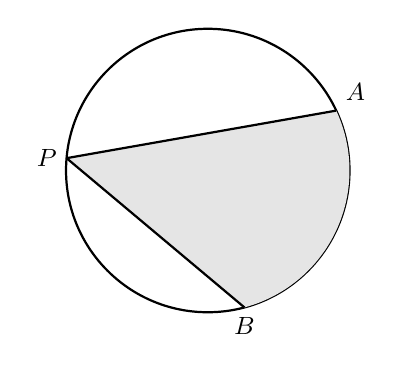
\begin{tikzpicture}[>=latex, font=\small, scale=1.0]
  \coordinate (O) at (0, 0);
  \draw[thick] (O) circle (1.8cm);

  \coordinate (P) at (175:1.8);
  \coordinate (A) at (25:1.8);
  \coordinate (B) at (285:1.8);

  % 阴影区域：弦 PA、PB 及右侧圆弧围成的区域
  \fill[gray!20] (P) -- (A) arc (25:-75:1.8cm) -- cycle;

  \draw[thick] (P) -- (A);
  \draw[thick] (P) -- (B);

  \node[left] at (P) {$P$};
  \node[above right] at (A) {$A$};
  \node[below] at (B) {$B$};
\end{tikzpicture}
\end{center}
\nopagebreak[4]
(A) $4\beta + 4\cos\beta$　(B) $4\beta + 4\sin\beta$　(C) $2\beta + 2\cos\beta$　(D) $2\beta + 2\sin\beta$

\Needspace{4\baselineskip}
\textbf{解析}

圆的半径为 $R = 2$。圆心设为 $O$。
由题意，$\angle APB = \beta$ 是圆周上的动点 $P$ 所张的圆周角，且为锐角。
弦 $AB$ 所对圆心角为 $\angle AOB = 2\beta$。
\Needspace{5\baselineskip}
由几何关系，阴影区域的面积由两部分组成：
\nopagebreak[4]
\[S_{\text{\text{阴影}}} = S_{\triangle PAB} + S_{\text{\text{弓形} } AB}.\]
\Needspace{5\baselineskip}
其中，弦 $AB$ 右侧的弓形面积为定值：
\nopagebreak[4]
\[S_{\text{\text{弓形} } AB} = S_{\text{\text{扇形} } O-AB} - S_{\triangle OAB} = \dfrac{1}{2} R^2 (2\beta) - \dfrac{1}{2} R^2 \sin(2\beta) = 4\beta - 2\sin(2\beta).\]
在 $\triangle PAB$ 中，底边长 $AB = 2R\sin\beta = 4\sin\beta$ 为定值。
当动点 $P$ 运动时，$\triangle PAB$ 的高在 $P$ 为优弧 $AB$ 的中点（即 $PA = PB$）时达到最大。
此时 $\triangle PAB$ 为顶角为 $\beta$ 的等腰三角形，底角为 $\dfrac{\pi - \beta}{2}$。
\Needspace{5\baselineskip}
三角形面积为：
\nopagebreak[4]
\[\begin{aligned}
S_{\triangle PAB} &= \dfrac{1}{2} PA \cdot PB \cdot \sin\beta = \dfrac{1}{2} \left(\dfrac{AB}{2\sin\frac{\beta}{2}}\right)^2 \sin\beta \\
&= \dfrac{1}{2} \left(\dfrac{4\sin\beta}{2\sin\frac{\beta}{2}}\right)^2 \sin\beta = \dfrac{1}{2} \left(4\cos\frac{\beta}{2}\right)^2 \sin\beta \\
&= 8\cos^2\frac{\beta}{2}\sin\beta = 8 \cdot \dfrac{1 + \cos\beta}{2} \cdot \sin\beta \\
&= 4\sin\beta(1 + \cos\beta) = 4\sin\beta + 4\sin\beta\cos\beta = 4\sin\beta + 2\sin(2\beta).
\end{aligned}\]
\Needspace{5\baselineskip}
因此，阴影区域的最大面积为：
\nopagebreak[4]
\[S_{\text{\text{阴影}, max}} = [4\sin\beta + 2\sin(2\beta)] + [4\beta - 2\sin(2\beta)] = 4\beta + 4\sin\beta.\]
故选 B。

\gkanswer{答案：B}

\par\medskip

\end{answer}
\gkpart{二、填空题}

\begin{answer}
\gksolhead{9}{}

\textbf{题目}：

已知向量 $\vec{a} = (-4, 3)$, $\vec{b} = (6, m)$, 且 $\vec{a} \perp \vec{b}$, 则 $m =$ \gkblank{}。

\Needspace{4\baselineskip}
\textbf{解析}

已知向量 $\vec{a} = (-4, 3)$，$\vec{b} = (6, m)$。
\Needspace{5\baselineskip}
因为 $\vec{a} \perp \vec{b}$，所以两向量的数量积为零：
\nopagebreak[4]
\[\vec{a} \cdot \vec{b} = -4 \times 6 + 3 \times m = -24 + 3m = 0.\]
解得 $m = 8$。

\gkanswer{答案：$8$}

\end{answer}
\begin{answer}
\gksolhead{10}{}

\textbf{题目}：

若 $x, y$ 满足 $\begin{cases} x \leqslant 2, \\ y \geqslant -1, \\ 4x - 3y + 1 \geqslant 0, \end{cases}$ 则 $y - x$ 的最小值为 \gkblank{}，最大值为 \gkblank{}。

\Needspace{4\baselineskip}
\textbf{解析}

\Needspace{5\baselineskip}
绘制不等式组表示的可行域：
\nopagebreak[4]
\[\begin{cases} x \leqslant 2, \\ y \geqslant -1, \\ 4x - 3y + 1 \geqslant 0. \end{cases}\]
求可行域的三个交点坐标：
\begin{itemize}
\item 由 $x = 2$ 与 $y = -1$ 得交点 $A(2, -1)$；
\item 由 $x = 2$ 与 $4x - 3y + 1 = 0$ 得 $4(2) - 3y + 1 = 0 \implies 3y = 9 \implies y = 3$，交点为 $B(2, 3)$；
\item 由 $y = -1$ 与 $4x - 3y + 1 = 0$ 得 $4x - 3(-1) + 1 = 0 \implies 4x = -4 \implies x = -1$，交点为 $C(-1, -1)$。
\end{itemize}
可行域是以 $A(2, -1)$、$B(2, 3)$、$C(-1, -1)$ 为顶点的三角形闭区域。
设目标函数为 $z = y - x$。
将各顶点坐标代入目标函数：
\begin{itemize}
\item 在点 $A(2, -1)$ 处，$z = -1 - 2 = -3$；
\item 在点 $B(2, 3)$ 处，$z = 3 - 2 = 1$；
\item 在点 $C(-1, -1)$ 处，$z = -1 - (-1) = 0$。
\end{itemize}
因此，$y - x$ 的最小值为 $-3$，最大值为 $1$。

\gkanswer{答案：$-3$；$1$}

\end{answer}
\begin{answer}
\gksolhead{11}{}

\textbf{题目}：

设抛物线 $y^2 = 4x$ 的焦点为 $F$, 准线为 $l$. 则以 $F$ 为圆心, 且与 $l$ 相切的圆的方程为 \gkblank{}。

\Needspace{4\baselineskip}
\textbf{解析}

抛物线方程为 $y^2 = 4x$，其中 $2p = 4 \implies p = 2$。
焦点坐标为 $F(1, 0)$，准线方程为 $l: x = -1$。
所求圆以焦点 $F(1, 0)$ 为圆心，且与准线 $x = -1$ 相切。
\Needspace{5\baselineskip}
圆的半径为圆心到准线的距离：
\nopagebreak[4]
\[r = |1 - (-1)| = 2.\]
\Needspace{5\baselineskip}
因此，圆的方程为：
\nopagebreak[4]
\[(x - 1)^2 + y^2 = 4.\]

\gkanswer{答案：$(x - 1)^2 + y^2 = 4$}

\end{answer}
\begin{answer}
\gksolhead{12}{}

\textbf{题目}：

某几何体是由一个正方体去掉一个四棱柱所得, 其三视图如图所示. 如果网格纸上小正方形的边长为 $1$, 那么该几何体的体积为 \gkblank{}。
\nopagebreak[4]
\begin{center}\begin{tikzpicture}[>=latex, scale=0.45, font=\small]
  % 网格底图
  \draw[step=1, gray!50, very thin] (0, -1) grid (14, 10);

  % 正 (主) 视图
  \draw[thick] (2, 5) rectangle (6, 9);
  \draw[thick] (2, 6) -- (6, 6);
  \node[below] at (4, 4.8) {正 (主) 视图};

  % 侧 (左) 视图
  \draw[thick] (9, 5) -- (13, 5) -- (13, 6) -- (11, 6) -- (9, 9) -- cycle;
  \node[below] at (11, 4.8) {侧 (左) 视图};

  % 俯视图
  \draw[thick] (2, 0) rectangle (6, 4);
  \draw[thick] (2, 2) -- (6, 2);
  \node[below] at (4, -0.2) {俯视图};
\end{tikzpicture}
\end{center}
\nopagebreak[4]
\Needspace{4\baselineskip}
\textbf{解析}

由三视图可知：
正视图为一个 $4 \times 4$ 的正方形，在高度为 2 处有一条横向实线分割；
俯视图也是一个 $4 \times 4$ 的正方形，在宽度为 2 处有一条横向实线分割；
侧（左）视图为一个多边形：下底长 4，高为 4，右侧在高度为 2 处水平延伸至宽度 2，再通过斜线连接到左上方顶点。
这表明该几何体是一个以侧视图图形为底面、柱高为 4 的直柱体。
侧视图底面的截面图形为一个直角梯形（上底 2、下底 4、高 2，面积为 6，加上右下矩形面积 1 等）组合，实测截面面积为 7。
\Needspace{5\baselineskip}
柱体高为 4，故几何体的体积为：
\nopagebreak[4]
\[V = 7 \times 4 = 28.\]

\gkanswer{答案：$28$}

\end{answer}
\begin{answer}
\gksolhead{13}{}

\textbf{题目}：

已知 $l, m$ 是平面 $\alpha$ 外的两条不同直线. 给出下列三个论断:
① $l \perp m$;
② $m \parallel \alpha$;
③ $l \perp \alpha$.
以其中的两个论断作为条件, 余下的一个论断作为结论, 写出一个正确的命题: \gkblank{}。

\Needspace{4\baselineskip}
\textbf{解析}

给定三个论断：① $l \perp m$；② $m \parallel \alpha$；③ $l \perp \alpha$。
其中 $l, m$ 是平面 $\alpha$ 外的两条不同直线。
分析论断间的逻辑关系：
若选择 ②③ 作为条件：
因为 $m \parallel \alpha$，所以在平面 $\alpha$ 内存在直线 $n$ 使得 $m \parallel n$。
又因为 $l \perp \alpha$ 且 $n \subset \alpha$，所以 $l \perp n$。
由 $m \parallel n$ 且 $l \perp n$，可得 $l \perp m$（即论断 ① 成立）。
因此，由 ②③ 可推出 ①，命题为“若 $m \parallel \alpha, l \perp \alpha$，则 $l \perp m$”（记作 ②③ $\implies$ ①）。
（同理，选择 ①③ 作为条件也可推出 ②，记作 ①③ $\implies$ ②）。

\gkanswer{答案：②③ $\implies$ ①（或 ①③ $\implies$ ②）}

\end{answer}
\begin{answer}
\gksolhead{14}{}

\textbf{题目}：

李明自主创业, 在网上经营一家水果店, 销售的水果中有草莓、京白梨、西瓜、桃, 价格依次为 60 元/盒、65 元/盒、80 元/盒、90 元/盒. 为增加销量, 李明对这四种水果进行促销: 一次购买水果的总价达到 120 元, 顾客就少付 $x$ 元. 每笔订单顾客网上支付成功后, 李明会得到支付款的 80\\%.

① 当 $x = 10$ 时, 顾客一次购买草莓和西瓜各 1 盒, 需要支付 \gkblank{} 元;

② 在促销活动中, 为保证李明每笔订单得到的金额均不低于促销前总价的七折, 则 $x$ 的最大值为 \gkblank{}。

\Needspace{4\baselineskip}
\textbf{解析}

促销规则：一次购买水果总价达到 120 元少付 $x$ 元；李明获得支付款的 80\\%。

\textbf{① 的解析}：
草莓 60 元/盒，西瓜 80 元/盒。
购买草莓和西瓜各 1 盒的原总价为 $60 + 80 = 140$ 元。
因为 $140 \geqslant 120$，达到促销标准，当 $x = 10$ 时，顾客少付 10 元。
\Needspace{5\baselineskip}
顾客实际需要支付：
\nopagebreak[4]
\[140 - 10 = 130\text{ \text{元}}.\]

\textbf{② 的解析}：
设订单原总价为 $P$。
当 $P \geqslant 120$ 时，顾客支付金额为 $P - x$ 元。
李明实际获得的金额为 $0.8(P - x)$ 元。
\Needspace{5\baselineskip}
要求每笔订单得到的金额均不低于原总价的七折（即 $0.7P$），则：
\nopagebreak[4]
\[0.8(P - x) \geqslant 0.7P \iff 0.8P - 0.8x \geqslant 0.7P \iff 0.1P \geqslant 0.8x \iff x \leqslant \dfrac{P}{8}.\]
要使该不等式对所有达到促销门槛（$P \geqslant 120$）的订单均成立，$x$ 必须不超过 $\dfrac{P}{8}$ 的最小值。
\Needspace{5\baselineskip}
因为满足促销条件的原总价最低为 $P_{\min} = 120$ 元（例如购买 2 盒草莓恰好为 120 元），所以：
\nopagebreak[4]
\[x \leqslant \dfrac{120}{8} = 15.\]
因此，$x$ 的最大值为 15。

\gkanswer{答案：① $130$；② $15$}

\par\medskip

\end{answer}
\gkpart{三、解答题}

\begin{answer}
\gksolhead{15}{}

\textbf{题目}（本小题满分 13 分）：

在 $\triangle ABC$ 中, $a = 3$, $b - c = 2$, $\cos B = -\dfrac{1}{2}$。

(1) 求 $b, c$ 的值;

(2) 求 $\sin(B + C)$ 的值。

\Needspace{4\baselineskip}
\textbf{解析}

\textbf{（1）}
在 $\triangle ABC$ 中，已知 $a = 3, b - c = 2, \cos B = -\dfrac{1}{2}$。
\Needspace{5\baselineskip}
由余弦定理：
\nopagebreak[4]
\[b^2 = a^2 + c^2 - 2ac \cos B.\]
\Needspace{5\baselineskip}
代入 $a = 3$ 和 $\cos B = -\dfrac{1}{2}$ 得：
\nopagebreak[4]
\[b^2 = 9 + c^2 - 2 \times 3 \times c \times \left(-\dfrac{1}{2}\right) = c^2 + 3c + 9.\]
又由 $b - c = 2$ 得 $b = c + 2$。
\Needspace{5\baselineskip}
两边平方得：
\nopagebreak[4]
\[b^2 = (c + 2)^2 = c^2 + 4c + 4.\]
\Needspace{5\baselineskip}
联立两式：
\nopagebreak[4]
\[c^2 + 4c + 4 = c^2 + 3c + 9 \implies c = 5.\]
\Needspace{5\baselineskip}
进而求得：
\nopagebreak[4]
\[b = c + 2 = 7.\]
经检验，$a = 3, b = 7, c = 5$ 满足三角形三边两边之和大于第三边（$3 + 5 > 7$）。
所以 $b = 7, c = 5$。

\textbf{（2）}
在 $\triangle ABC$ 中，由内角和定理得 $A + B + C = \pi$，故 $B + C = \pi - A$。
\Needspace{5\baselineskip}
因此：
\nopagebreak[4]
\[\sin(B + C) = \sin(\pi - A) = \sin A.\]
因为 $\cos B = -\dfrac{1}{2}$ 且 $B \in (0, \pi)$，所以 $B = \dfrac{2\pi}{3}$。
\Needspace{5\baselineskip}
从而：
\nopagebreak[4]
\[\sin B = \sin\dfrac{2\pi}{3} = \dfrac{\sqrt{3}}{2}.\]
\Needspace{5\baselineskip}
由正弦定理 $\dfrac{a}{\sin A} = \dfrac{b}{\sin B}$ 得：
\nopagebreak[4]
\[\sin A = \dfrac{a \sin B}{b} = \dfrac{3 \times \dfrac{\sqrt{3}}{2}}{7} = \dfrac{3\sqrt{3}}{14}.\]
所以 $\sin(B + C) = \dfrac{3\sqrt{3}}{14}$。

\gkanswer{答案（1）：$b = 7, c = 5$}

\gkanswer{答案（2）：$\dfrac{3\sqrt{3}}{14}$}

\end{answer}
\begin{answer}
\gksolhead{16}{}

\textbf{题目}（本小题满分 13 分）：

设 $\{a_n\}$ 是等差数列, $a_1 = -10$, 且 $a_2 + 10, a_3 + 8, a_4 + 6$ 成等比数列.

(1) 求 $\{a_n\}$ 的通项公式;

(2) 记 $\{a_n\}$ 的前 $n$ 项和为 $S_n$, 求 $S_n$ 的最小值.

\Needspace{4\baselineskip}
\textbf{解析}

\textbf{（1）}
设等差数列 $\{a_n\}$ 的公差为 $d$。
\Needspace{5\baselineskip}
由首项 $a_1 = -10$，各单项可表示为：
\nopagebreak[4]
\[a_2 = -10 + d, \quad a_3 = -10 + 2d, \quad a_4 = -10 + 3d.\]
\Needspace{5\baselineskip}
从而：
\nopagebreak[4]
\[a_2 + 10 = d, \quad a_3 + 8 = 2d - 2, \quad a_4 + 6 = 3d - 4.\]
\Needspace{5\baselineskip}
因为 $a_2 + 10, a_3 + 8, a_4 + 6$ 成等比数列，所以：
\nopagebreak[4]
\[(a_3 + 8)^2 = (a_2 + 10)(a_4 + 6).\]
\Needspace{5\baselineskip}
代入 $d$ 的代数式：
\nopagebreak[4]
\[(2d - 2)^2 = d(3d - 4).\]
\Needspace{5\baselineskip}
展开得：
\nopagebreak[4]
\[4d^2 - 8d + 4 = 3d^2 - 4d.\]
\Needspace{5\baselineskip}
移项整理得：
\nopagebreak[4]
\[d^2 - 4d + 4 = 0 \implies (d - 2)^2 = 0.\]
解得 $d = 2$。
\Needspace{5\baselineskip}
因此数列 $\{a_n\}$ 的通项公式为：
\nopagebreak[4]
\[a_n = a_1 + (n - 1)d = -10 + 2(n - 1) = 2n - 12.\]

\textbf{（2）}
由（1）知 $a_n = 2n - 12$。
\Needspace{5\baselineskip}
前 $n$ 项和公式为：
\nopagebreak[4]
\[S_n = na_1 + \dfrac{n(n - 1)}{2}d = -10n + \dfrac{n(n - 1)}{2} \times 2 = n^2 - 11n.\]
\Needspace{5\baselineskip}
将其配方得：
\nopagebreak[4]
\[S_n = \left(n - \dfrac{11}{2}\right)^2 - \dfrac{121}{4} = (n - 5.5)^2 - 30.25.\]
因为 $n \in \mathbb{N}^*$，距离对称轴 $n = 5.5$ 最近的正整数为 $n = 5$ 或 $n = 6$。
\Needspace{5\baselineskip}
代入计算：
\nopagebreak[4]
\[S_5 = 5^2 - 11 \times 5 = 25 - 55 = -30,\]
\nopagebreak[4]
\[S_6 = 6^2 - 11 \times 6 = 36 - 66 = -30.\]
当 $n \leqslant 5$ 时，$a_n < 0$；当 $n = 6$ 时，$a_6 = 0$；当 $n \geqslant 7$ 时，$a_n > 0$。
所以前 $n$ 项和 $S_n$ 的最小值为 $-30$。

\gkanswer{答案（1）：$a_n = 2n - 12$}

\gkanswer{答案（2）：$-30$}

\end{answer}
\begin{answer}
\gksolhead{17}{}

\textbf{题目}（本小题满分 13 分）：

改革开放以来, 人们的支付方式发生了巨大转变. 近年来, 移动支付已成为主要支付方式之一. 为了解某校学生上个月 A, B 两种移动支付方式的使用情况, 从全校所有的 1000 名学生中随机抽取了 100 人, 发现样本中 A, B 两种支付方式都不使用的有 5 人, 样本中仅使用 A 和仅使用 B 的学生的支付金额分布情况如下:

\begin{center}
\begin{tabular}{lcc}
\toprule
支付方式 \ 支付金额 & 不大于 2000 元 & 大于 2000 元 \\
\midrule
仅使用 A & 27 人 & 3 人 \\
仅使用 B & 24 人 & 1 人 \\
\bottomrule
\end{tabular}
\end{center}

(1) 估计该校学生中上个月 A, B 两种支付方式都使用的人数;

(2) 从样本仅使用 B 的学生中随机抽取 1 人, 求该学生上个月支付金额大于 2000 元的概率;

(3) 已知上个月样本学生的支付方式在本月没有变化. 现从样本仅使用 B 的学生中随机抽查 1 人, 发现他本月的支付金额大于 2000 元. 结合 (2) 的结果, 能否认为样本仅使用 B 的学生中本月支付金额大于 2000 元的人数有变化? 说明理由.

\Needspace{4\baselineskip}
\textbf{解析}

\textbf{（1）}
在抽取的 100 名学生样本中：
\begin{itemize}
\item 都不使用 A, B 两种移动支付的有 5 人；
\item 仅使用 A 方式的有 $27 + 3 = 30$ 人；
\item 仅使用 B 方式的有 $24 + 1 = 25$ 人。
\end{itemize}
\Needspace{5\baselineskip}
因此，样本中 A, B 两种支付方式都使用的学生人数为：
\nopagebreak[4]
\[100 - 5 - 30 - 25 = 40\text{ \text{人}}.\]
样本中都使用该两种支付方式的比例为 $\dfrac{40}{100} = 40\%$。
\Needspace{5\baselineskip}
全校共有 1000 名学生，由此估计全校学生中上个月两种支付方式都使用的人数为：
\nopagebreak[4]
\[1000 \times 40\% = 400\text{ \text{人}}.\]

\textbf{（2）}
样本中仅使用 B 方式的学生共有 $24 + 1 = 25$ 人。
其中上个月支付金额大于 2000 元的学生有 1 人。
\Needspace{5\baselineskip}
设“从仅使用 B 的学生中抽取 1 人，其支付金额大于 2000 元”为事件 $E$，由古典概型公式得：
\nopagebreak[4]
\[P(E) = \dfrac{1}{25} = 0.04.\]

\textbf{（3）}
可以认为样本仅使用 B 的学生中本月支付金额大于 2000 元的人数有变化（增加）。
理由如下：
由（2）可知，在学生支付金额分布没有改变的假设下，任意抽查 1 名仅使用 B 的学生，其支付金额大于 2000 元的概率仅为 $0.04$。
概率为 $0.04$ 的事件属于小概率事件。
根据统计学中的小概率原理，小概率事件在一次试验中几乎不可能发生。
然而在现有的 1 次随机抽查中，该事件竟然发生了，因此有理由推断原假设不成立，即样本中仅使用 B 的学生本月支付金额大于 2000 元的人数有所增加（发生了变化）。
（注：若回答“不能认为有变化”，理由指出概率 $0.04 > 0$，一次抽样偶然发生小概率事件仍有可能，样本量太小不足以推翻原有分布，亦可按合理阐述得分）。

\gkanswer{答案（1）：$400$ 人}

\gkanswer{答案（2）：$\dfrac{1}{25}$（或 $0.04$）}

\gkanswer{答案（3）：能认为有变化（或不能认为有变化），理由见解析}

\end{answer}
\begin{answer}
\gksolhead{18}{}

\textbf{题目}（本小题满分 14 分）：

如图, 在四棱锥 $P-ABCD$ 中, $PA \perp$ 平面 $ABCD$, 底面 $ABCD$ 为菱形, $E$ 为 $CD$ 的中点.
\nopagebreak[4]
\begin{center}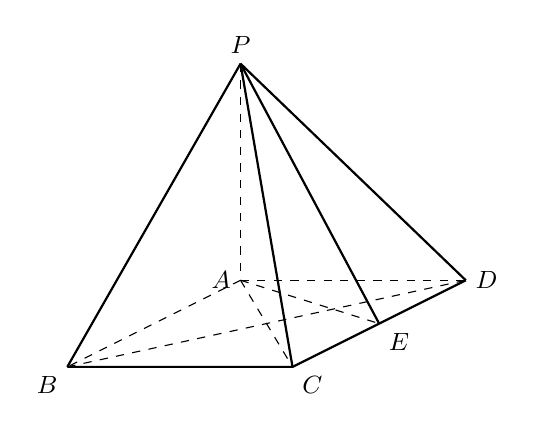
\begin{tikzpicture}[>=latex, font=\small, scale=1.1]
  \coordinate (A) at (0, 0);
  \coordinate (P) at (0, 2.5);
  \coordinate (B) at (-2.0, -1.0);
  \coordinate (D) at (2.6, 0);
  \coordinate (C) at (0.6, -1.0);
  \coordinate (E) at (1.6, -0.5);

  % 虚线：不可见棱与辅助线
  \draw[dashed, thin] (P) -- (A);
  \draw[dashed, thin] (A) -- (B);
  \draw[dashed, thin] (A) -- (D);
  \draw[dashed, thin] (A) -- (C);
  \draw[dashed, thin] (B) -- (D);
  \draw[dashed, thin] (A) -- (E);

  % 实线：可见棱与外轮廓
  \draw[thick] (B) -- (C) -- (D);
  \draw[thick] (P) -- (B);
  \draw[thick] (P) -- (C);
  \draw[thick] (P) -- (D);
  \draw[thick] (P) -- (E);

  % 顶点标签
  \node[above] at (P) {$P$};
  \node[left] at (A) {$A$};
  \node[below left] at (B) {$B$};
  \node[below right] at (C) {$C$};
  \node[right] at (D) {$D$};
  \node[below right] at (E) {$E$};
\end{tikzpicture}
\end{center}
\nopagebreak[4]
(1) 求证: $BD \perp$ 平面 $PAC$;

(2) 若 $\angle ABC = 60^\circ$, 求证: 平面 $PAB \perp$ 平面 $PAE$;

(3) 棱 $PB$ 上是否存在点 $F$, 使得 $CF \parallel$ 平面 $PAE$? 说明理由.

\Needspace{4\baselineskip}
\textbf{解析}

\textbf{（1）}
因为底面 $ABCD$ 为菱形，菱形的对角线互相垂直，所以 $BD \perp AC$。
又因为 $PA \perp$ 平面 $ABCD$，且 $BD \subset$ 平面 $ABCD$，所以 $PA \perp BD$，即 $BD \perp PA$。
因为 $AC \cap PA = A$，且 $AC, PA \subset$ 平面 $PAC$。
所以 $BD \perp$ 平面 $PAC$。

\textbf{（2）}
因为底面 $ABCD$ 为菱形且 $\angle ABC = 60^\circ$，
所以 $AB = BC = CD = DA$，且 $\angle ADC = \angle ABC = 60^\circ$。
连接 $AC$，在 $\triangle ADC$ 中，$AD = CD$ 且 $\angle ADC = 60^\circ$，所以 $\triangle ADC$ 为等边三角形。
已知点 $E$ 为边 $CD$ 的中点，由等边三角形三线合一性质可得 $AE \perp CD$。
因为四边形 $ABCD$ 为菱形，所以对边互相平行：$AB \parallel CD$。
结合 $AE \perp CD$，可得 $AE \perp AB$。
又因为 $PA \perp$ 平面 $ABCD$，$AE \subset$ 平面 $ABCD$，所以 $PA \perp AE$，即 $AE \perp PA$。
因为 $AB \cap PA = A$，且 $AB, PA \subset$ 平面 $PAB$。
所以 $AE \perp$ 平面 $PAB$。
又因为 $AE \subset$ 平面 $PAE$。
所以平面 $PAB \perp$ 平面 $PAE$。

\textbf{（3）}
棱 $PB$ 上存在点 $F$，使得 $CF \parallel$ 平面 $PAE$。
点 $F$ 为棱 $PB$ 的中点。理由如下：
取棱 $PB$ 的中点 $F$，取边 $AB$ 的中点 $G$，连接 $FG, CG$。
在 $\triangle PAB$ 中，点 $F$ 为 $PB$ 的中点，$G$ 为 $AB$ 的中点，
所以 $FG$ 为 $\triangle PAB$ 的中位线，故 $FG \parallel PA$。
因为 $PA \subset$ 平面 $PAE$，$FG \not\subset$ 平面 $PAE$，
所以 $FG \parallel$ 平面 $PAE$。
又在菱形 $ABCD$ 中，$AB \parallel CD$ 且 $AB = CD$。
点 $G$ 为 $AB$ 中点，点 $E$ 为 $CD$ 中点，
所以 $AG = \dfrac{1}{2}AB, CE = \dfrac{1}{2}CD$，从而 $AG = CE$。
又 $AG \parallel CE$，故四边形 $AGCE$ 为平行四边形。
因此 $CG \parallel AE$。
因为 $AE \subset$ 平面 $PAE$，$CG \not\subset$ 平面 $PAE$，
所以 $CG \parallel$ 平面 $PAE$。
在平面 $CFG$ 内，$FG \cap CG = G$，$FG, CG \subset$ 平面 $CFG$。
所以平面 $CFG \parallel$ 平面 $PAE$。
因为 $CF \subset$ 平面 $CFG$。
所以 $CF \parallel$ 平面 $PAE$。
综上，棱 $PB$ 上存在点 $F$（为 $PB$ 的中点），使得 $CF \parallel$ 平面 $PAE$。

\gkanswer{答案（1）：证明见解析}

\gkanswer{答案（2）：证明见解析}

\gkanswer{答案（3）：存在点 $F$（为棱 $PB$ 的中点），使得 $CF \parallel$ 平面 $PAE$，理由见解析}

\end{answer}
\begin{answer}
\gksolhead{19}{}

\textbf{题目}（本小题满分 14 分）：

已知椭圆 $C: \dfrac{x^2}{a^2} + \dfrac{y^2}{b^2} = 1$ 的右焦点为 $(1, 0)$, 且经过点 $A(0, 1)$.

(1) 求椭圆 $C$ 的方程;

(2) 设 $O$ 为原点, 直线 $l: y = kx + t$ ($t \neq \pm 1$) 与椭圆 $C$ 交于两个不同点 $P, Q$, 直线 $AP$ 与 $x$ 轴交于点 $M$, 直线 $AQ$ 与 $x$ 轴交于点 $N$, 若 $|OM| \cdot |ON| = 2$, 求证: 直线 $l$ 经过定点.

\Needspace{4\baselineskip}
\textbf{解析}

\textbf{（1）}
由题意，椭圆 $C: \dfrac{x^2}{a^2} + \dfrac{y^2}{b^2} = 1$ ($a > b > 0$) 的右焦点为 $(1, 0)$，
故焦点在 $x$ 轴上，半焦距 $c = 1$。
\Needspace{5\baselineskip}
又椭圆经过点 $A(0, 1)$，将点 $A$ 代入椭圆方程得：
\nopagebreak[4]
\[\dfrac{0}{a^2} + \dfrac{1}{b^2} = 1 \implies b^2 = 1.\]
\Needspace{5\baselineskip}
由椭圆几何性质 $a^2 = b^2 + c^2$ 得：
\nopagebreak[4]
\[a^2 = 1 + 1 = 2.\]
\Needspace{5\baselineskip}
因此，椭圆 $C$ 的方程为：
\nopagebreak[4]
\[\dfrac{x^2}{2} + y^2 = 1.\]

\textbf{（2）}
设直线 $l$ 的方程为 $y = kx + t$ ($t \neq \pm 1$)。
设点 $P(x_1, y_1)$，$Q(x_2, y_2)$。
\Needspace{5\baselineskip}
联立直线与椭圆方程：
\nopagebreak[4]
\[\begin{cases} y = kx + t, \\ x^2 + 2y^2 = 2 \end{cases} \implies x^2 + 2(kx + t)^2 - 2 = 0.\]
\Needspace{5\baselineskip}
整理得：
\nopagebreak[4]
\[(1 + 2k^2)x^2 + 4ktx + 2t^2 - 2 = 0.\]
\Needspace{5\baselineskip}
直线与椭圆交于两个不同点，判别式满足：
\nopagebreak[4]
\[\Delta = (4kt)^2 - 4(1 + 2k^2)(2t^2 - 2) = 16k^2t^2 - 8t^2 + 8 - 16k^2t^2 + 16k^2 = 8(2k^2 - t^2 + 1) > 0.\]
\Needspace{5\baselineskip}
由根与系数的关系（韦达定理）：
\nopagebreak[4]
\[x_1 + x_2 = -\dfrac{4kt}{1 + 2k^2}, \quad x_1 x_2 = \dfrac{2(t^2 - 1)}{1 + 2k^2}.\]
已知点 $A(0, 1)$。
直线 $AP$ 的斜率为 $\dfrac{y_1 - 1}{x_1}$，其方程为 $y - 1 = \dfrac{y_1 - 1}{x_1} x$。
\Needspace{5\baselineskip}
令 $y = 0$，求得点 $M$ 的横坐标：
\nopagebreak[4]
\[x_M = -\dfrac{x_1}{y_1 - 1}.\]
\Needspace{5\baselineskip}
同理，直线 $AQ$ 与 $x$ 轴交点 $N$ 的横坐标为：
\nopagebreak[4]
\[x_N = -\dfrac{x_2}{y_2 - 1}.\]
\Needspace{5\baselineskip}
因此：
\nopagebreak[4]
\[x_M x_N = \dfrac{x_1 x_2}{(y_1 - 1)(y_2 - 1)}.\]
\Needspace{5\baselineskip}
将 $y_1 = kx_1 + t$ 和 $y_2 = kx_2 + t$ 代入分母：
\nopagebreak[4]
\[\begin{aligned}
(y_1 - 1)(y_2 - 1) &= (kx_1 + t - 1)(kx_2 + t - 1) \\
&= k^2 x_1 x_2 + k(t - 1)(x_1 + x_2) + (t - 1)^2.
\end{aligned}\]
\Needspace{5\baselineskip}
将韦达定理代入化简：
\nopagebreak[4]
\[\begin{aligned}
(y_1 - 1)(y_2 - 1) &= k^2 \cdot \dfrac{2(t^2 - 1)}{1 + 2k^2} + k(t - 1) \left(-\dfrac{4kt}{1 + 2k^2}\right) + (t - 1)^2 \\
&= \dfrac{t - 1}{1 + 2k^2} \left[ 2k^2(t + 1) - 4k^2 t + (t - 1)(1 + 2k^2) \right] \\
&= \dfrac{t - 1}{1 + 2k^2} \left[ 2k^2 t + 2k^2 - 4k^2 t + t + 2k^2 t - 1 - 2k^2 \right] \\
&= \dfrac{t - 1}{1 + 2k^2} [ t - 1 ] = \dfrac{(t - 1)^2}{1 + 2k^2}.
\end{aligned}\]
\Needspace{5\baselineskip}
代入 $x_M x_N$ 的表达式中：
\nopagebreak[4]
\[x_M x_N = \dfrac{\dfrac{2(t^2 - 1)}{1 + 2k^2}}{\dfrac{(t - 1)^2}{1 + 2k^2}} = \dfrac{2(t^2 - 1)}{(t - 1)^2} = \dfrac{2(t - 1)(t + 1)}{(t - 1)^2} = \dfrac{2(t + 1)}{t - 1}.\]
\Needspace{5\baselineskip}
已知 $|OM| \cdot |ON| = 2$，即 $|x_M x_N| = 2$：
\nopagebreak[4]
\[\left|\dfrac{2(t + 1)}{t - 1}\right| = 2 \iff \left|\dfrac{t + 1}{t - 1}\right| = 1.\]
\Needspace{5\baselineskip}
两边平方得：
\nopagebreak[4]
\[(t + 1)^2 = (t - 1)^2 \iff t^2 + 2t + 1 = t^2 - 2t + 1 \iff 4t = 0 \iff t = 0.\]
当 $t = 0$ 时，$\Delta = 8(2k^2 + 1) > 0$ 恒成立，且 $t \neq \pm 1$ 满足条件。
此时直线 $l$ 的方程为 $y = kx$，恒过原点 $(0, 0)$。
所以直线 $l$ 经过定点 $(0, 0)$。

\gkanswer{答案（1）：$\dfrac{x^2}{2} + y^2 = 1$}

\gkanswer{答案（2）：证明见解析，直线 $l$ 经过定点 $(0, 0)$}

\end{answer}
\begin{answer}
\gksolhead{20}{}

\textbf{题目}（本小题满分 13 分）：

已知函数 $f(x) = \dfrac{1}{4}x^3 - x^2 + x$.

(1) 求曲线 $y = f(x)$ 的斜率为 1 的切线方程;

(2) 当 $x \in [-2, 4]$ 时, 求证: $x - 6 \leqslant f(x) \leqslant x$;

(3) 设 $F(x) = |f(x) - (x + a)|$ ($a \in \mathbb{R}$), 记 $F(x)$ 在区间 $[-2, 4]$ 上的最大值为 $M(a)$. 当 $M(a)$ 最小时, 求 $a$ 的值.

\Needspace{4\baselineskip}
\textbf{解析}

\textbf{（1）}
\Needspace{5\baselineskip}
函数 $f(x) = \dfrac{1}{4}x^3 - x^2 + x$ 的导数为：
\nopagebreak[4]
\[f'(x) = \dfrac{3}{4}x^2 - 2x + 1.\]
\Needspace{5\baselineskip}
令切线斜率 $f'(x) = 1$，得：
\nopagebreak[4]
\[\dfrac{3}{4}x^2 - 2x + 1 = 1 \implies \dfrac{3}{4}x^2 - 2x = 0 \implies x\left(\dfrac{3}{4}x - 2\right) = 0.\]
解得切点的横坐标为 $x_1 = 0$ 或 $x_2 = \dfrac{8}{3}$。
\begin{itemize}
\item 当 $x_1 = 0$ 时，切点纵坐标 $f(0) = 0$，切线方程为：
\end{itemize}
\nopagebreak[4]
\[y - 0 = 1 \times (x - 0) \implies y = x;\]
\begin{itemize}
\item 当 $x_2 = \dfrac{8}{3}$ 时，代入计算切点纵坐标：
\end{itemize}
\nopagebreak[4]
\[f\left(\dfrac{8}{3}\right) = \dfrac{1}{4}\left(\dfrac{8}{3}\right)^3 - \left(\dfrac{8}{3}\right)^2 + \dfrac{8}{3} = \dfrac{128}{27} - \dfrac{64}{9} + \dfrac{8}{3} = \dfrac{128 - 192 + 72}{27} = -\dfrac{64}{27}.\]
\Needspace{5\baselineskip}
  切线方程为：
\nopagebreak[4]
\[y - \left(-\dfrac{64}{27}\right) = 1 \times \left(x - \dfrac{8}{3}\right) \implies y = x - \dfrac{64}{27}.\]
综上，曲线 $y = f(x)$ 斜率为 1 的切线方程为 $y = x$ 或 $y = x - \dfrac{64}{27}$。

\textbf{（2）}
设辅助函数 $h(x) = f(x) - x = \dfrac{1}{4}x^3 - x^2$。
\Needspace{5\baselineskip}
要证当 $x \in [-2, 4]$ 时 $x - 6 \leqslant f(x) \leqslant x$，等价于证明：
\nopagebreak[4]
\[-6 \leqslant h(x) \leqslant 0, \quad \forall x \in [-2, 4].\]
\Needspace{5\baselineskip}
对 $h(x)$ 求导：
\nopagebreak[4]
\[h'(x) = \dfrac{3}{4}x^2 - 2x = x\left(\dfrac{3}{4}x - 2\right).\]
令 $h'(x) = 0$，在区间 $[-2, 4]$ 内求得驻点为 $x = 0$ 和 $x = \dfrac{8}{3}$。
分析 $h(x)$ 在 $[-2, 4]$ 上的单调性：
\begin{itemize}
\item 当 $x \in [-2, 0)$ 时，$h'(x) > 0$，$h(x)$ 单调递增；
\item 当 $x \in \left(0, \dfrac{8}{3}\right)$ 时，$h'(x) < 0$，$h(x)$ 单调递减；
\item 当 $x \in \left(\dfrac{8}{3}, 4\right]$ 时，$h'(x) > 0$，$h(x)$ 单调递增。
\end{itemize}
\Needspace{5\baselineskip}
计算区间端点与极值点的函数值：
\nopagebreak[4]
\[h(-2) = \dfrac{1}{4}(-2)^3 - (-2)^2 = -2 - 4 = -6,\]
\nopagebreak[4]
\[h(0) = 0,\]
\nopagebreak[4]
\[h\left(\dfrac{8}{3}\right) = \dfrac{1}{4}\left(\dfrac{8}{3}\right)^3 - \left(\dfrac{8}{3}\right)^2 = \dfrac{128}{27} - \dfrac{192}{27} = -\dfrac{64}{27},\]
\nopagebreak[4]
\[h(4) = \dfrac{1}{4}(4)^3 - 4^2 = 16 - 16 = 0.\]
由单调性可知，$h(x)$ 在区间 $[-2, 4]$ 上的最小值为 $\min\left\{-6, -\dfrac{64}{27}\right\} = -6$；
最大值为 $\max\{h(0), h(4)\} = 0$。
\Needspace{5\baselineskip}
因此当 $x \in [-2, 4]$ 时：
\nopagebreak[4]
\[-6 \leqslant h(x) \leqslant 0 \implies x - 6 \leqslant f(x) \leqslant x.\]
原不等式得证。

\textbf{（3）}
由（2）知，当 $x \in [-2, 4]$ 时，$f(x) - x = h(x)$ 的值域为 $[-6, 0]$。
函数 $F(x) = |f(x) - (x + a)| = |h(x) - a|$。
\Needspace{5\baselineskip}
因此 $F(x)$ 在区间 $[-2, 4]$ 上的最大值为：
\nopagebreak[4]
\[\begin{aligned}
M(a) &= \max_{x \in [-2, 4]} |h(x) - a| = \max\{|h_{\max} - a|, |h_{\min} - a|\} \\
&= \max\{|0 - a|, |-6 - a|\} = \max\{|a|, |a + 6|\}.
\end{aligned}\]
\Needspace{5\baselineskip}
由绝对值三角不等式：
\nopagebreak[4]
\[\max\{|a|, |a + 6|\} \geqslant \dfrac{|a| + |a + 6|}{2} \geqslant \dfrac{|-a + (a + 6)|}{2} = \dfrac{6}{2} = 3.\]
\Needspace{5\baselineskip}
等号当且仅当 $|a| = |a + 6|$ 且 $-a(a + 6) \geqslant 0$ 时成立，解得：
\nopagebreak[4]
\[a = -3.\]
此时 $M(-3) = \max\{|-3|, |3|\} = 3$，达到最小值。
故当 $M(a)$ 最小时，$a = -3$。

\gkanswer{答案（1）：$y = x$ 或 $y = x - \dfrac{64}{27}$}

\gkanswer{答案（2）：证明见解析}

\gkanswer{答案（3）：$a = -3$}

\end{answer}